\documentclass[10pt]{article}

% Packages
\usepackage{graphicx}
\usepackage{amsmath}
\usepackage{hyperref}
\usepackage{geometry}
\usepackage{changepage}
\usepackage{fancyhdr}
\usepackage{tocloft}
\usepackage{titlesec}
\usepackage{lastpage}
\usepackage{caption}
\usepackage{tabularx}
\usepackage{array}
\usepackage{multicol}

\captionsetup[figure]{
    font={it, small},
    labelfont=bf,
    labelsep=period,
    justification=centering,
    singlelinecheck=false
}

\captionsetup[table]{
    font={it, small},
    labelfont=bf,
    labelsep=period,
    justification=centering,
    singlelinecheck=false
}

\titleformat{\section}
{\normalsize\bfseries}
{\thesection \, \textbar}
{0.5em}
{}

\titleformat{\subsection}
{\normalsize\bfseries}
{\thesubsection \, \textbar}
{0.5em}
{}

\geometry{a4paper, margin=1in}

\fancyhf{}
\fancyfoot[L]{
    \scriptsize\bfseries
    Department of Computer Engineering\\
    Chulalongkorn University
}

\renewcommand{\headrulewidth}{0pt}
\renewcommand{\footrulewidth}{0.5pt}
\renewcommand{\cftsecaftersnum}{.}
\renewcommand{\arraystretch}{1.75}

\newcolumntype{Y}{>{\centering\arraybackslash}X}
\newcolumntype{L}{>{\raggedright\arraybackslash}X}
\newcolumntype{R}{>{\raggedleft\arraybackslash}X}

\sloppy
\begin{document}
    \pagestyle{plain}
    \begin{titlepage}
        \noindent
{\footnotesize
Computer Engineering Capstone Project Proposal
\par}

\vspace{0.3cm}

\noindent
{\Large\bfseries
Utilization of High Precision Software System
\par}

\noindent
{\Large\bfseries
for Development of Interactive Entertainment Media
\par}

\vspace{0.4cm}

\noindent
{\small
Tapaneeya Odmung   \, \textbar \,
Wachirawich Kanil  \, \textbar \,
Pranesh Ingkanunt  \, \textbar \,
Rangsiman Jearuksa
\par}

\vspace{0.3cm}

\noindent
{\scriptsize
Department of Computer Engineering, Chulalongkorn University, Bangkok, Thailand
\par}

\vspace{0.3cm}

\noindent
{\scriptsize
\textbf{Advisor:}
Asst. Prof. Vishnu Kotrajaras (vishnu@cp.eng.chula.ac.th),
Kamin Kolyutsakul %(something@somewhere.com)
\par}

\vspace{0.3cm}

\noindent
{\scriptsize
\textbf{Keywords:}
high-performance computing,
computer graphics,
real-time rendering,
parallel processing,
software architecture,
game engine
\par}

\vspace{0.3cm}

\noindent
{\normalsize \today \par}

\vspace{0.5cm}

\begin{center}
    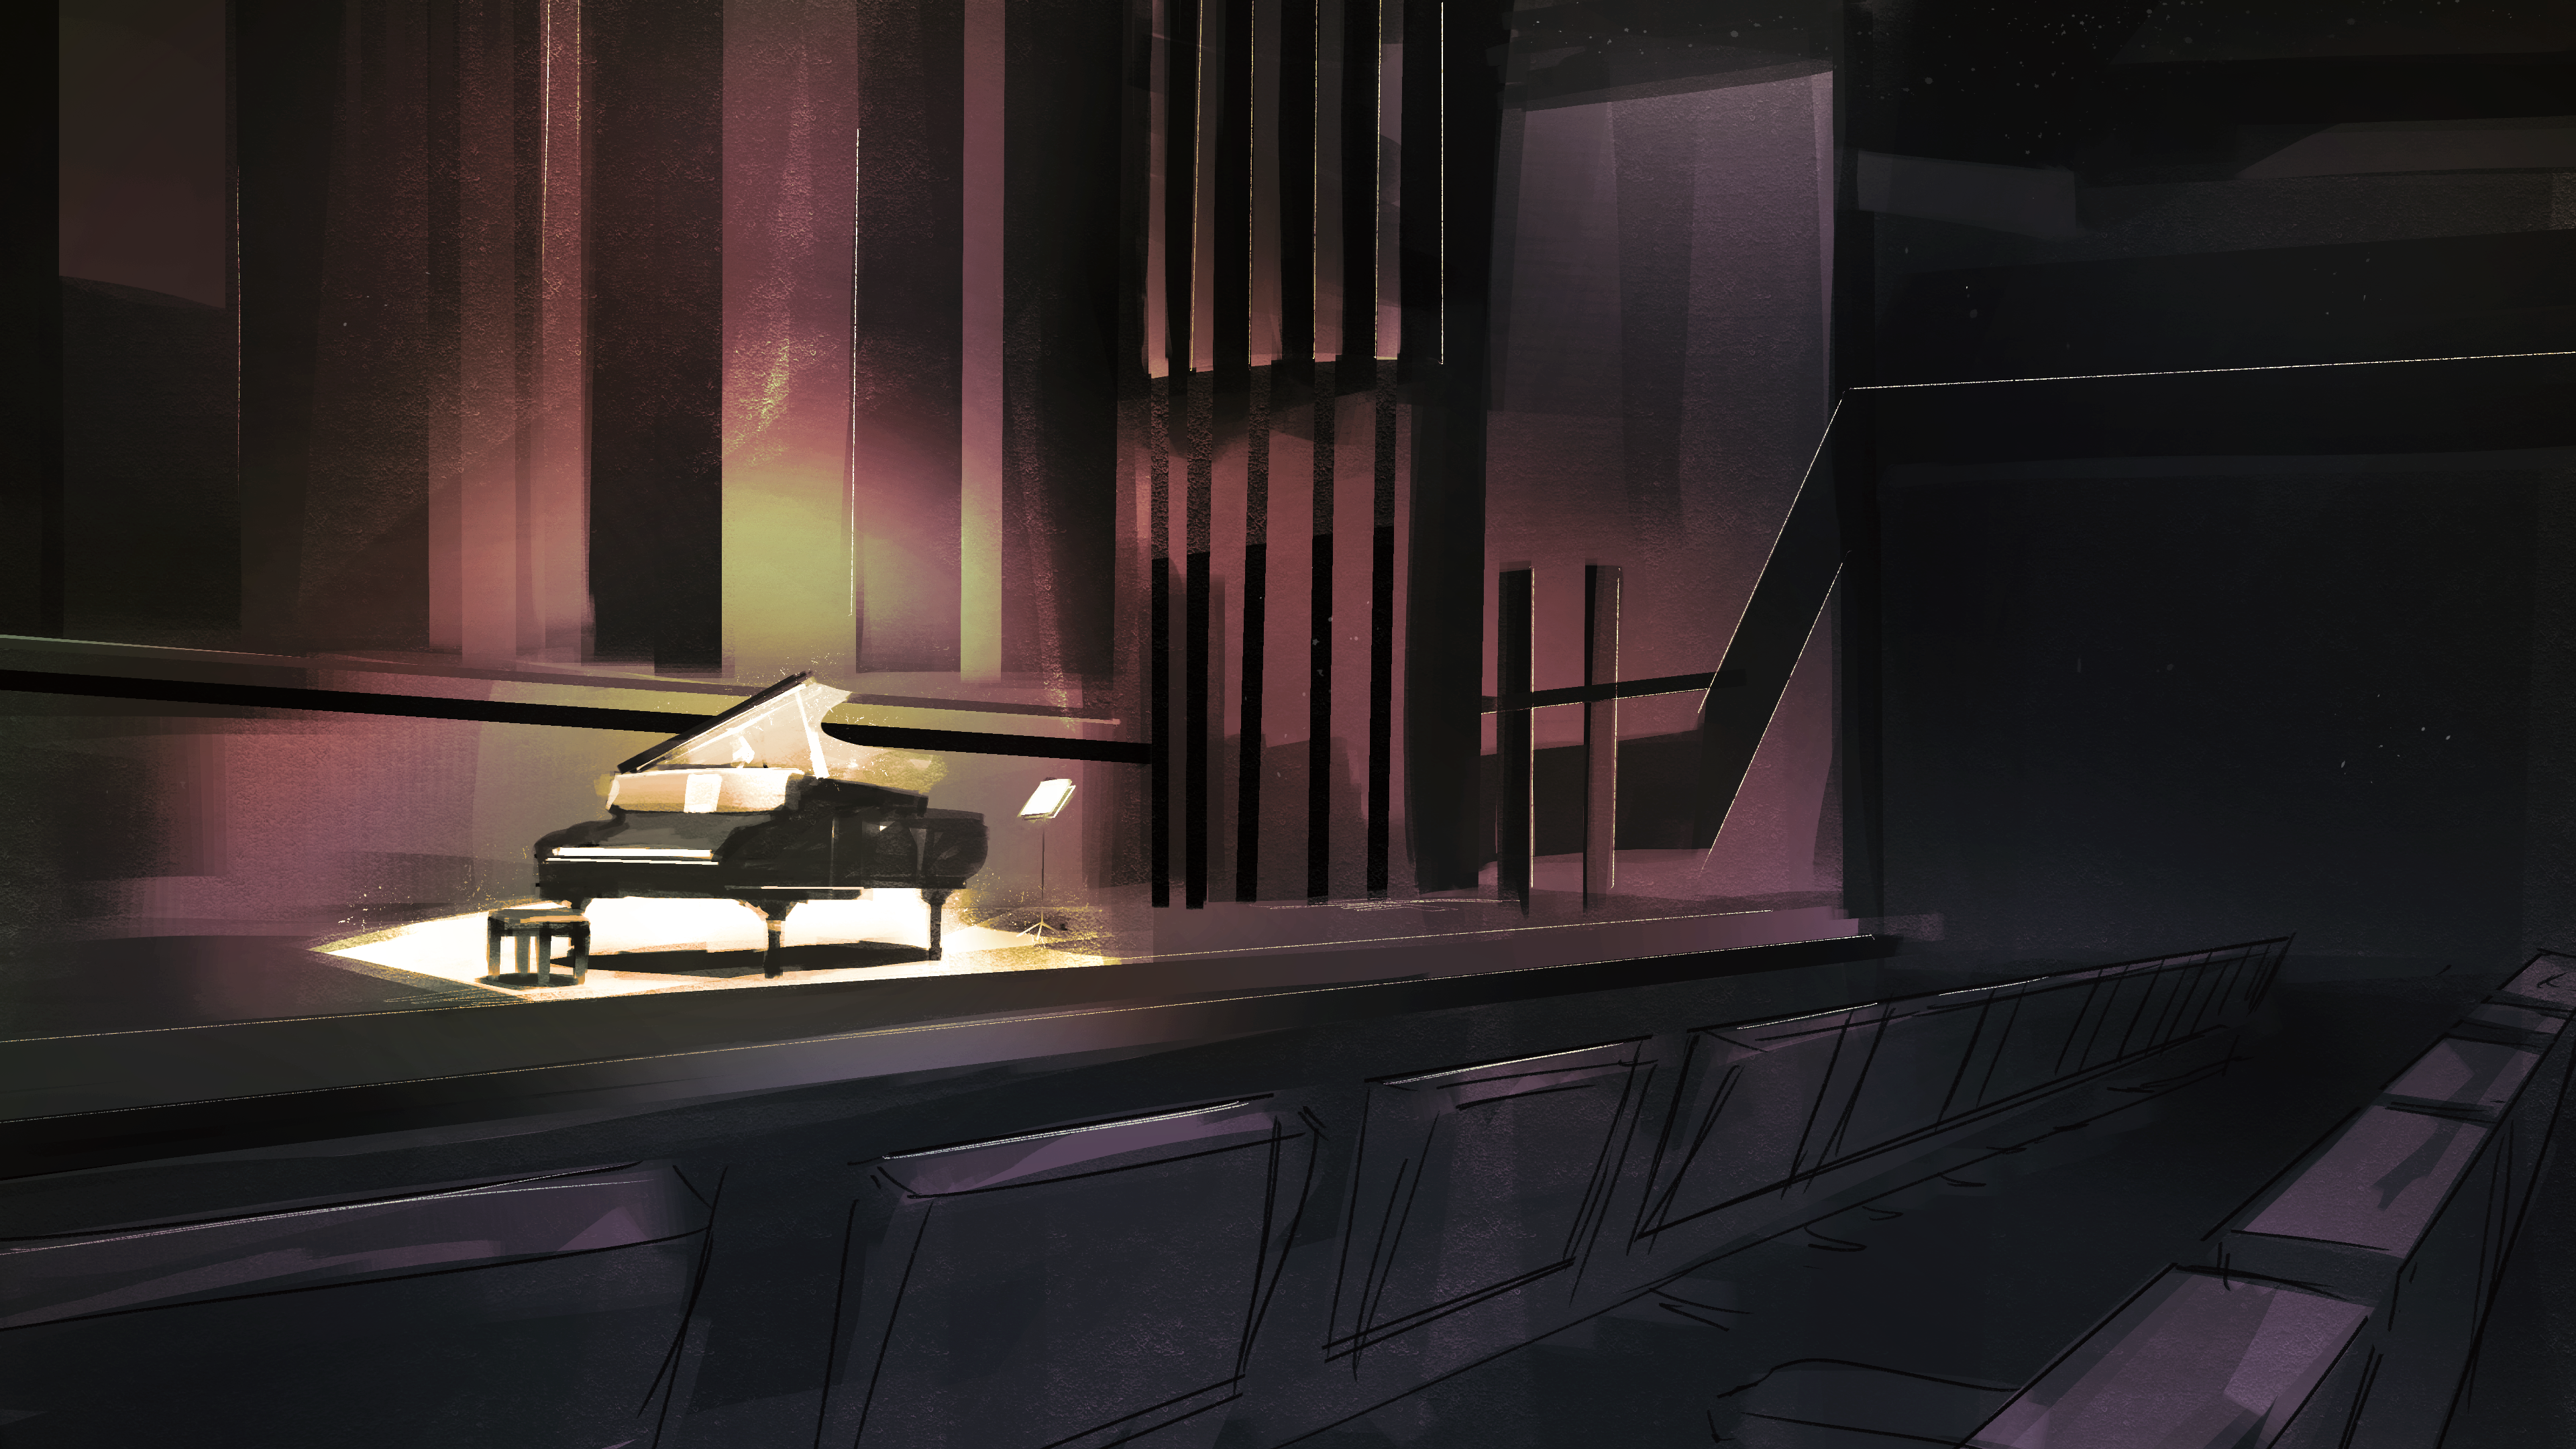
\includegraphics[width=\textwidth, keepaspectratio]{images/title}
\end{center}

%{\rule{\textwidth}{0.5px}\par}
%\vspace{-0.4cm}
        \noindent
        {\rule{\textwidth}{0.5px}\par}
        \vspace{-0.4cm}
        \begin{adjustwidth}{0.5cm}{0.5cm}
    \section*{\normalsize Abstract}
    \vspace{-0.3cm}
    \normalsize
    This project focuses on addressing the lack of a versatile and high-performance general purpose interactive media
    creation framework, which is important due to the prevalence of interactive media in academic and medical contexts.
    The objectives of this project are to analyze the limitations of existing game engine architectures, particularly
    in their usage of creating general purpose interactive media, as well as to explore alternative paradigms and
    finally develop a framework that can streamline its creation with minimal development costs and maintaining high
    performance and usability across various domains.
    To achieve these objectives, the proposed solution involves an operating-system-like game engine, integrating
    the Entity-Component-Structure framework with operating systems concepts, while utilizing aggressive C++ compile-time
    optimization to increase performance.
    \\\\
    The methodology will include C++20, DirectX 11, and Windows API to design and analyze the system, and
    GoogleTest to validate it.
    The outcomes we expected from this project are a proposal, a deliverable prototype, and a system documentation,
    which we expected will provide industrial benefits to future creations of interactive media.

\end{adjustwidth}
        \noindent
        {\rule{\textwidth}{0.5px}\par}
    \end{titlepage}

    \pagestyle{fancy}
    \pagenumbering{roman}
    \fancyfoot[R]{\thepage}

    \addcontentsline{toc}{section}{Contents}
    \tableofcontents
    \thispagestyle{fancy}
    \newpage

    \fancyfoot[R]{
        \thepage\ of \pageref{tag:end}
    }
    \pagenumbering{arabic}
    \setcounter{page}{1}

    \begin{multicols}{2}
        \raggedcolumns
        \section{Introduction}
\label{sec:introduction}

\subsection{Background \& Motivation}
\label{subsec:background-and-motivation}

In recent years, interactive media has become increasingly more integrated into modern society.
It has appeared within games, applications, and Virtual Reality (VR) with usage covering
many fields, including within academic and medical contexts.
As such media continues to develop in scale and complexity, its performance demands have intensified.
The growth in hardware performance is not enough to keep up with this demand, creating a challenge for
creators and system designers alike.
\\\\
Current interactive media is usually created by relying on game engines, such as Unity, Godot, and Unreal Engine,
as a software framework.
However, these game engines were originally designed for game development and were not built for the more
general applications.
This mismatch motivates the need to create such a system that is built optimally for these new demands,
while remaining highly optimized in terms of performance for various tasks.

\subsection{Problem Statement}
\label{subsec:problem-statement}

Existing game engines are not suitable for the creation of general-purpose interactive media.
Their architecture uses the traditional object-oriented programming (OOP) paradigm, which introduces
certain constraints and limitations on flexibility, scalability, and performance outside game contexts.
\\\\
In response, many companies have resorted to developing proprietary systems from scratch to meet their specific requirements.
This practice, however, leads to delays in development while accruing unnecessary costs.
The problem, therefore, is that there lacks a sufficiently versatile and high-performance framework that can
efficiently support the development of general-purpose interactive media.

\subsection{Objectives}
\label{subsec:objectives}

\begin{enumerate}
    \item To analyze the limitations of existing game engine architectures, particularly in relation to general-purpose interactive applications.
    \item To explore alternative architectural paradigms that could offer improved performance and flexibility over conventional OOP-based designs.
    \item To propose and develop a framework that can streamline the creation of interactive media while reducing development costs and maintaining high performance.
    \item To evaluate the proposed framework through game development as a case study to demonstrate its effectiveness in real-world scenarios.
\end{enumerate}

\subsection{Scope \& Limitations}
\label{subsec:scope-and-limitation}
This project is intended to develop high-precision software for creation of interactive media, which can receive user inputs and respond accordingly.
In order to achieve this goal, we need to have control on our system as much as possible.
That means everything on this system will rely on the Operating System's library and
C++ standard library (STL) function that is proven to be zero-cost abstractions, according to the
International Organization for Standardization (ISO). If specified to be up to the implementation,
we will refer to Microsoft Visual C++ implementation of STL\@.
\\\\
As a case study, we will implement a rhythm game with bullet hell systems and
compete in Game Talent Showcase competition hosted by Thai Game Software Industry Association (TGA)
using as few libraries as possible.

\subsection{Expected Benefits}
\label{subsec:expected-benefits}

\begin{enumerate}
    \item A clearer understanding of current game design architectures and its limitations on the development of general-purpose interactive media.
    \item A structured analysis of alternative design paradigms that may overcome these limitations.
    \item A practical framework that simplifies the development of interactive systems across multiple application domains.
    \item Enhanced adaptability and performance in future interactive media platforms.
\end{enumerate}
        \section{Related Work}
\label{sec:related-work}

\subsection{Review of Existing Knowledge}
\label{subsec:review-of-existing-knowledge}

\subsection{Comparison with Existing Systems}
\label{subsec:comparison-with-existing-systems}

\subsection{Gap Analysis}
\label{subsec:gap-analysis}

\subsection{Linkage to Project}
\label{subsec:linkage-to-project}
        \section{System Design}
\label{sec:system-design}

\subsection{System Overview}
\label{subsec:system-overview}

\subsubsection*{Engine Design}

The project's core engine design, as stated before, will use an ECS framework that registers and
determines components and system dependencies at compile-time.
The declaration of a single ECS instance that registers all components and systems would result in
wasteful usage of memory and projected performance decreases due to the large variety of components involved.
As such, we have opted to use multiple smaller ECS instances that each take control of a smaller part of the game.
We refer to these smaller ECS instances, alongside the data necessary to register related components and systems,
as well as compute and store initial data into those instances, as scenes.
Communications between scenes, such as the data transfer when creating a new scene, are facilitated through
a manager, which will also execute the registered systems during the main game loop.
DirectX 11 is used for the rendering of the game with the use of a custom rendering pipeline implementation.
User input is collected through the Windows API\@.

\subsubsection*{Game Design}

The project’s core game design will involve combining rhythm games and bullet hell games into a hybrid game
structured around distinct but smoothly transitioning phases,
thus requiring a seamless transition between the two, creating a revolutionary take on hybrid games.
Having that both of the games hugely relied on great optimization, as with a little disruption,
it can cause a fatal unintended mistake for the player inciting frustration;
therefore, the design of the game must be made cautiously.
\\\\
The bullet hell section is mostly composed of large amounts of bullets and particles
while great performance is still required to attain the player’s fluidity of movement.
To achieve this, an ECS architecture is highly favoured as opposed to object-oriented
since the high amount of entities can be handled more efficiently with it.
Entities of the system are composed of player, bullets, boss, enemies, background and effects
utilizing shared components such as position, velocity, sprite, shader, etc.
Each system will be executed every frame thus handling the entity movement,
collision check and input allowing it to handle all the bullets in a frame efficiently.
Such systems consist of a player system, movement system, collision system, particle system and much more.
The core mechanics is for each frame, the input was processed to control the player system
while the collision system will check each ongoing colliding entity by calling each entity with a collider component
and computing if they are colliding with which entity.
Then, the corresponding function will be triggered to apply change to the state such as the player taking damage and making change to the player’s health UI\@.
Moreover, the movement system computes the next frame position to render, and lastly, the animation system will render the right frame of the animation at the correct time.
\\\\
Rhythm games require precise timing and precision to catch the note at the right time,
very little or next to none of the optimization issues can be tolerated as a result.
However, ECS architecture is powerful enough to handle all the requirements
such as notes quantities and an accurate time tracking device centralized by a single system.
With entities as simple as notes, lanes and judgement, components are widely adjustable with speed, timing and judgement.
In addition, the system design is fairly simple as the input system and judgement system is centralized and the note system moves all notes called.
Along with the bullet hell section, they contain backgrounds that are adjustable by shader and particle effects.
The core mechanic revolves around spawning the notes at the right time as set up.
Then, each note will be called by the movement system to calculate the position of the sprite.
However, the real logic of the note is being computed by another system that reduces its timing to be compared in the judgement system.
Lastly, the judgement system calls the corresponding system to handle whether if the note has been well-time pressed and sending responses to the player.
\\\\
Transitioning between both gameplay proves to be a great challenge design-wise
because it has to be smooth and seamless enough to not disrupt the precision-hungry gameplay of both games.
Firstly, in the whole game process, only one game scene may be rendered to minimize time to transition
as the whole scene will be loaded and initiated only once from the start.
If the transition is happening, the gameplay should be frozen and any progress should not be counted during the process,
allowing the player to get ready to adjust their gameplay smoothly.
The transition's animation has to telegraph the player clearly to make them aware that the gameplay is going to be changed
as the timer UI counts down to inform the duration and delay of the transition precisely.
Lastly, the screen changing the gameplay rendered has to be transition creative by splitting the screen in two and slowly expanding the next gameplay.
To achieve this, a line animation system is used to express animation of the transition
and the Game Transition System will be triggered if the state has been changed rendering the new gameplay for a section of the screen expanding until full.
\\\\
A biggest concern of the system is the control of the rhythm game’s charts and bullet hell’s patterns
needing to be not too exhaustingly difficult to control as both games require vast amounts of complicated pattern and timing design.
A solution proposed would be to create our own scripting language and a corresponding compiler such as a chart file.
Practicing these techniques makes designing and implementing charts and patterns much easier
allowing more complex and challenging design and features.
\\\\
To complete a game, a narrative device should be implemented to make the game more immersive and enjoyable;
the proposed gameplay would be a 2D side-scrolling style that allows players to choose a level and progress the story of the gameplay.
Additionally, explorations are added to the game such as interacting with an interactable such as NPC, or objects, obtaining new in-game items and accessing new areas.
Such requirements must be implemented with an entirely new system.
Interactable and solid collision components are needed to be implemented along with the new system, for example, new movement system, interact system and area load system.
\\\\
Lastly, using ECS, UI entities are being rendered concurrently in a higher priority by default.
The entities will have a position, text, sprite and animation components and are created organizedly using functions for each set of UIs.
For sound and music in the game, just like UIs as each is assigned to its own entity holding a tag or trigger to be played on an instance sound system at the right time.
Finally, the cutscene could be added as a video format to be rendered in an instance video player system.



\subsection{Components}
\label{subsec:components}

The system is a self-contained application, but interfacing with a keyboard and mouse is required for its operation.



\subsection{Constraints Considered}
\label{subsec:constraints-considered}

Due to the usage of the Windows API and DirectX 11, the system is to be operated and published only on
the Windows operating system.

\subsection{Diagrams}
\label{subsec:diagrams}

\vspace{0.5cm}

\begin{figure}[h]
    \centering
    \includegraphics[width=\columnwidth, keepaspectratio]{images/taskmanager}
    \caption{A diagram showing how task manager works}
    \label{fig:taskmanager}
\end{figure}

\vspace{0.5cm}

Describe how task manager works here.

\vspace{0.5cm}

\begin{figure}[h]
    \centering
    \includegraphics[width=\columnwidth, keepaspectratio]{images/scenemanager}
    \caption{A diagram showing how scene manager works}
    \label{fig:scenemanager}
\end{figure}

\vspace{0.5cm}

\noindent Describe how scene manager works here.

\vspace{0.5cm}

\begin{figure}[h]
    \centering
    \includegraphics[width=\columnwidth, keepaspectratio]{images/scenemanager2}
    \caption{A diagram showing how scene manager transfers data from old scene to new scene}
    \label{fig:scenemanager2}
\end{figure}

\vspace{0.5cm}

\noindent Describe how scene manager transfers data here.

\vspace{0.5cm}

\begin{figure}[h]
    \centering
    \includegraphics[width=\columnwidth, keepaspectratio]{images/gameflow}
    \caption{A diagram showing scene flow of the game prototype}
    \label{fig:gameflow}
\end{figure}

\vspace{0.5cm}

\noindent Figure~\ref{fig:gameflow} shows how the scenes in our game should flow.
The game starts from the main menu scene where the player can choose to enter the game or exit.
After the player chooses to enter the game, the game's world scene will be loaded.
The world is a 2D side-scrolling scene where the player can explore and choose levels to play.
There will be objects across the world which act as stages that the player can interact with to 
enter the level.
When the player interacts with a stage object, the game will transition to pre-stage scene, where 
they can select which instrument to use in the level.
Each instrument represents a different difficulty level.
The player can choose to start the level with the selected instrument or return to the world.
Once the player starts the level, the game will transition to the main gameplay scene.
The gameplay scene consists of both bullet hell and rhythm game phases.
In this scene, as the level begins, the player will start with bullet hell phase.
The player must avoid incoming obstacles from the enemy and survive throughout the phase.
Each hit taken will reduce the player's health.
If the player's health reaches zero at any point, the gameplay will end, failing the level.
After surviving the for a certain amount of time, the game will transition to rhythm game phase.
In this phase, the player must hit the notes in time with the music to attack the enemy.
A gauge is displayed at the top of the screen to show the player's progress in defeating the enemy.
Each successful note hit will slightly fill the gauge, while missed notes will deplete it.
The player must fill the gauge above a certain threshold to defeat the enemy and complete the level.
Then, the game will transition back to bullet hell phase again.
This cycle continues until the song ends or the player is defeated first.
If the player successfully fills the gauge above the threshold by the end of the song, the player wins.
Otherwise, it is considered a draw.
After the gameplay ends, regardless if the player wins, loses or draws, the game will transition to results 
scene, displaying the player's performance statistics.
Then, the player will return to the world scene to continue exploring or choose another level.
    \end{multicols}
    \begin{multicols}{1}
        \section{Teamwork Plan}
\label{sec:teamwork-plan}
\subsection{Roles and Responsibilities}
\label{subsec:roles-and-responsibilities}

\vspace{1em}

\centering
%    \begin{tabularx}{\columnwidth}{X X}
%        Name & Roles\\
%        \hline
%        Tapaneeya Odmung & Project Lead \newline System Software Architecture \newline Operating System Level Software Engineer\\
%        Wachirawich Kanil & System Software Architecture \newline User Level Software Engineer\\
%        Pranesh Ingkanunt & Gameplay Design \newline Game Programming \newline Gameplay Software Architecture\\
%        Rangsiman Jearuksa & Gameplay Design \newline Game Programming \newline Graphic Software Engineer\\
%        \hline
%    \end{tabularx}
\renewcommand{\arraystretch}{1.75}

\newcolumntype{Y}{>{\centering\arraybackslash}X}
\newcolumntype{L}{>{\raggedright\arraybackslash}X}
\newcolumntype{R}{>{\raggedleft\arraybackslash}X}

\small
\begin{minipage}{\textwidth}
    \begin{tabularx}{\textwidth}{|L|L|L|}
        \hline
        \textbf{Role} & \textbf{Name} & \textbf{Responsibilities} \\
        \hline
        Project Lead & - Tapaneeya Odmung & Project Planning, Define System Scope, Communication \\
        System Software Architecture & {- Tapaneeya Odmung \newline - Wachirawich Kanil} & Design Engine \\
        Gameplay Design & {- Pranesh Ingkanunt \newline - Rangsiman Jearuksa} & Design Gameplay \\
        Gameplay Software Engineer & {- Pranesh Ingkanunt \newline - Rangsiman Jearuksa} & Program Game \\
        Graphic Software Engineer & {- Tapaneeya Odmung \newline - Rangsiman Jearuksa} & Program Graphic \\
        Operating System Software Engineer & - Tapaneeya Odmung & Program Operating System Level Communication \\
        User Level Software Engineer & - Wachirawich Kanil & Program User Communication Level \\
        Gameplay Software Architecture & - Pranesh Ingkanunt & Design Gameplay Architecture \\
        \hline
    \end{tabularx}
    \captionof{table}{Roles and Resposibility}
\end{minipage}
\label{tab:table}
    \end{multicols}
    \vspace{0.5em}
    \begin{multicols}{2}
        \raggedcolumns
        \subsection{Collaborative Plan}
\label{subsec:collaborative-plan}
The way we plan to work together is to have a group meeting for updating progress and planning on Friday of every week.
We also have a meeting with the advisor on Thursday of every week.
If there is a need to be absent, every person needs to clearly state so beforehand.
Each system planning will be planned as sprints with durations of two weeks per each iteration.
After every iteration, we will have a reflection on the first Friday after the end of iteration.
For meeting, everyone on the team has selected to have meetings in online format on Discord.
\\\\
For project source code management, we will be using Git Version Control System and using GitHub as
a remote repository.
The project source code will contain only system source code, game source code, document, report and report image only.
For game resources will need to be downloaded outside the repository.
\\\\
We will be using Cmake as a build system to allow team members to work easily with any text editor.
We will also be using clangd as a formatter in order to have a consistent coding style.
MSVC is used as a main system compiler such that we target Windows Operating System specifically.
Although we allow any text editor to use within this project, Clion by JetBrains is preferred.

\subsection{Task Coverage}
\label{subsec:task-coverage}

\subsection*{Project Lead}
This is a person who will manage and plan the project.
The main task of this person is to create a systematic plan for the project which is tangible and able to lead to finish product.
Not only that, this person also needs to communicate and also contact insiders and outsiders as needed.
Also, this person must be able to understand every person on a team and be able to find a suitable solution to make
the work go smoothly as much as possible.
\\\\
Since this team is a small team, the project lead must be able to direct the project direction and understand the image
of the final product so that they can achieve the most beneficial outcome for the team.

\subsection*{System Software Architect}
This is a person who is responsible for our system design.
The responsibility for this person is that they must be able to design an architecture which is
suitable for the needs of the software.
They must also create a good work environment for the team to work
with using this system in the future.

\subsection*{Gameplay Designer}
This person is the person whose responsibility is to design a game which can test whether
the system is working as intended or not.

\subsection*{Game Software Engineer}
This is a person whose task is to implement the game according to gameplay design within the
structure planned by the Gameplay Software Architect.

\subsection*{Graphic Software Engineer}
This person is a person who works on creating graphic which has high fidelity and also works
on optimization the graphic section of the software such as GPU Memory Management.

\subsection*{Operating System Software Engineer}
This is a person who creates an Application Programming Interface (API) to communicate with
the operating system safely and optimally.
Also, this person must ensure the software security and memory safety.

\subsection*{User Level Software Engineer}
This is who creates an API for users to write software on this system.
The person in charge must be able to create an API that is easy to implement and use.

\subsection*{Gameplay Software Architecture}
This person is a person who designs the system flow of a game to ensure good user experience
and also optimal data flow within the game system.

\subsection{Workload Balance}
\label{subsec:workload-balance}
    Since this project is really large and requires highly specialized personnel, each task was assigned
    to each person with the intent for them to be the master of that aspect of the system.
    Each of the tasks has their own set of challenges and requires very deep understanding.
    This means every person got to have their own hard and easy tasks where, on higher-level management,
    it can be inferred that the workload is already balanced because of the need of specialty.
    \end{multicols}
    \newpage
    \begin{multicols}{1}
        \section{Timeline}
\label{sec:timeline}
\vspace{1em}
\centering
\small
\begin{minipage}{\textwidth}
    \begin{tabularx}{\textwidth}{|L|L|L|}
        \hline
        \textbf{Week} & \textbf{Task / Milestone} & \textbf{Deliverable} \\
        \hline
        Week 1\, \textendash \, 2 & Literature Review \& background study & Draft background \& problem statement \\
        Week 3\, \textendash \, 4 & Problem definition \& objectives & Problem statement \& objectives \\
        Week 5\, \textendash \, 7 & System-level design \& tool selection & Draft design diagram \& tool list \\
        Week 8\, \textendash \, 10 & Proposal Writing & Draft report \\
        Week 11\, \textendash \, 12 & Proposal revision (advisor feedback) & Revised report \\
        Week 13\, \textendash \, 14 & Proposal presentation preparation & Slides \\
        Week 15 & Proposal presentation & Final report \& slides \\
        \hline
    \end{tabularx}
    \captionof{table}{Timeline}
\end{minipage}
\label{tab:timeline}
    \end{multicols}
    \vspace{0.5em}
%    \begin{multicols}{2}
%        \raggedcolumns
%        \subsection{Week 1\,\textendash\,2}
\label{subsec:timeline-week1-2}

\subsection{Week 3\,\textendash\,4}
\label{subsec:timeline-week3-4}

\subsection{Week 5\,\textendash\,7}
\label{subsec:timeline-week5-7}

\subsection{Week 8\,\textendash\,10}
\label{subsec:timeline-week8-10}

\subsection{Week 11\,\textendash\,12}
\label{subsec:timeline-week11-12}

\subsection{Week 13\,\textendash14}
\label{subsec:timeline-week13-14}

\subsection{Week 15}
\label{subsec:timeline-week15}
%    \end{multicols}
    \begin{multicols}{1}
        \section{Planned Work}
\label{sec:planned-work}

\vspace{1em}
\centering
\small
\begin{minipage}{\textwidth}
    \begin{tabularx}{\textwidth}{|L|L|L|}
        \hline
        \textbf{Week} & \textbf{Task / Milestone} & \textbf{Deliverable} \\
        \hline
        Week 1\, \textendash \, 2 & Window creation \& system \& gameplay design & Empty window \& design draft \\
        Week 3\, \textendash \, 4 & Directx initialization \& API \& concept art & Render image on screen \& game design document \\
        Week 5\, \textendash \, 7 & Thread management \& finalize system design \& gameplay system design &  N-buffering multithreading system design \& final system draft \& gameplay design draft \\
        Week 8\, \textendash \, 10 & Implement user level system \& gameplay implementation & Update rendering on screen \& gameplay testing on cli \\
        Week 11\, \textendash \, 12 & Optimization \& testing \& final report draft & Final report draft \\
        Week 13\, \textendash \, 14 & Final presentation preparation \& report revision & Presentation slide draft \& Final report revised \\
        Week 15 & Final presentation & Final report \& slides \\
        \hline
    \end{tabularx}
    \captionof{table}{Planned Work}
\end{minipage}
\label{tab:planned-work}
    \end{multicols}
    \vspace{0.5em}
    \newpage
    \begin{multicols}{2}
        \raggedcolumns
%        \subsection{Week 1\,\textendash\,2}
\label{subsec:planned-week1-2}

\subsection{Week 3\,\textendash\,4}
\label{subsec:planned-week3-4}

\subsection{Week 5\,\textendash\,7}
\label{subsec:planned-week5-7}

\subsection{Week 8\,\textendash\,10}
\label{subsec:planned-week8-10}

\subsection{Week 11\,\textendash\,12}
\label{subsec:planned-week11-12}

\subsection{Week 13\,\textendash\,14}
\label{subsec:planned-week13-14}

\subsection{Week 15}
\label{subsec:planned-week15}

        \section{Ethic, Privacy, and Professional Consideration}
\label{sec:ethic-privacy-and-professional-consideration}

\subsection{Plagiarism Check}
\label{subsec:plagiarism-check}

\subsection{Credibility of Information}
\label{subsec:credibility-of-information}

\subsection{Intellectual Property \& Law}
\label{subsec:intellectual-property-and-law}
    \end{multicols}

    \onecolumn
    \fancyfoot[R]{\thepage}
    \pagenumbering{alph}

    \addcontentsline{toc}{section}{References}
    \bibliographystyle{ieeetr}
    \bibliography{refs}
    \newpage

    % -- Appendix if needed (which you will) -- %
    \appendix
    \renewcommand{\thesection}{\Alph{section}}
    \titleformat{\section}
    {\normalsize\bfseries}
    {Appendix \thesection \, \textbar}
    {0.5em}
    {}

    \makeatletter
    \renewcommand{\listoffigures}{
        \begingroup
        \let\old@makecaption\@makecaption
        \renewcommand{\@makecaption}[2]{##2\\}
        \parindent\z@
        \refstepcounter{section}
        \section*{Appendix \thesection \, \textbar \vspace{0.5em} List of Figures}
        \label{sec:appendix-list-of-figures}
        \addcontentsline{toc}{section}{Appendix \thesection. List of Figures}
        \@starttoc{lof}
        \let\old@makecaption\@makecaption
        \endgroup
    }

    \renewcommand{\listoftables}{
        \begingroup
        \let\old@makecaption\@makecaption
        \renewcommand{\@makecaption}[2]{##2\\}
        \parindent\z@
        \refstepcounter{section}
        \section*{Appendix \thesection \, \textbar \vspace{0.5em} List of Tables}
        \label{sec:appendix-list-of-tables}
        \addcontentsline{toc}{section}{Appendix \thesection. List of Tables}
        \@starttoc{lot}
        \let\old@makecaption\@makecaption
        \endgroup
    }
    \makeatother

    \listoffigures

    \listoftables
    \refstepcounter{section}
\section*{Appendix \thesection \, \textbar \vspace{0.5em} Feasibility}
\label{sec:appendix-feasibility}
\addcontentsline{toc}{section}{Appendix \thesection: Feasibility}%

\begin{enumerate}
    \item Technical Feasibility\\
    Each member of the team has experience and specialized skills in different areas of the project, 
    including software development, system architecture, game design, and graphics programming.
    This team structure ensures that all aspects of the project are covered by knowledgeable individuals.
    The project utilizes C++20, DirectX 11, and Windows API, which are well-documented and widely used technologies, with no other third-party libraries required.

    \item Schedule Feasibility\\
    The proposed timeline shows the parallel nature of the tasks, allowing each member to work on their assigned tasks simultaneously.
    Upon consideration of estimated workloads and potential challenges, the timeline appears achievable and is expected to be met within the second semester.

    \item Organizational Feasibility\\
    The project aims to provide tools and resources to help users creating interactive media in an efficient manner.
    Due to the robust architecture of the system, it can be easily extended and modified to accommodate future needs and requirements.

\end{enumerate}
    \refstepcounter{section}
\section*{Appendix \thesection \, \textbar \vspace{0.5em} Document Standard}
\label{sec:appendix-document-standard}
\addcontentsline{toc}{section}{Appendix \thesection. Document Standard}

This document is typeset in LaTeX using a custom standard designed for clarity, consistency, and professional presentation. The format emphasizes readability in both digital and printed form while supporting structured technical writing. The main standards are as follows:
\subsection*{1. Document Class and Layout}
The proposal is based on the article class with a 10-point font size on A4 paper. Page margins are set to 1 inch on all sides for balanced spacing and printing compatibility.
\subsection*{2. Typography and Sectioning}
The document uses normal-sized body text with bold section and subsection titles. Each section title is prefixed by its number and separated by a vertical bar for clear visual hierarchy (e.g., “2 | System Design”).
The layout alternates between single-column and two-column formats depending on content density — technical sections such as \textit{Design} and \textit{Ethics} are two-column for compactness, while detailed tables and timelines are presented in single-column layout for readability.
\subsection*{3. Headers and Footers}
All pages include a footer containing the department name and university on the left and the page number on the right. A thin horizontal rule separates the footer from the main text. Page numbering is shown in the format “\textit{current of total}” after the table of contents.
\subsection*{4. Captions and Figures}
Figure and table captions use small italic text with bold labels, followed by a period separator (e.g., “Figure 3. System Architecture”). Captions are centered and consistently formatted to maintain visual balance across columns.
\subection*{5. Tables and Column Types}
The tabularx package is used to create flexible tables that automatically adjust to the page width. Three custom column types are defined:
\begin{itemize}
    \item
    L for left-aligned text
    \item
    R for right-aligned text
    \item
    Y for centered text
    The line spacing inside tables is slightly increased (1.75×) for better readability in printed form.
    \end{itemize}
\subsection*{6. Page Style and Numbering}
Preliminary pages (title, abstract, and table of contents) use Roman numerals, while the main content uses Arabic numerals. Appendix pages are labeled alphabetically (A, B, C, etc.). Headers are omitted to maintain a clean layout.
\subsection*{7. Table of Contents and Structure}
The table of contents lists all major sections, references, and appendices. Each section and subsection is clearly numbered for easy navigation.
\subsection*{8. References}
References are formatted using the IEEE Transactions style (ieeetr), which is standard for engineering and computer science research. The bibliography section is automatically generated and included in the table of contents.
\subsection*{9. Appendices}
Appendices are styled consistently with the main document but relabeled alphabetically (e.g., “Appendix A | List of Figures”). Lists of figures and tables are customized to display caption titles only for compactness. Additional appendices may include feasibility analysis, code of conduct, and other supplementary materials.
\item
\subsection*{10. Compilation and Packages}
The document uses standard LaTeX packages for layout and styling, including:
\begin{itemize}
    \item
    geometry for margin control
    \item
    fancyhdr for footer customization
    \item
    titlesec for section formatting
    \item
    multicol for multi-column layout
    \item
    graphicx for image inclusion
    \item
    tabularx and array for table management
    \item
    hyperref for internal linking and references
    \end{itemize}

This formatting standard is chosen to ensure that the proposal is visually organized, technically clear, and easily extensible for later reports such as the progress and final project documentation.
    \refstepcounter{section}
\section*{Appendix \thesection \, \textbar \vspace{0.5em} Coding Standard}
\label{sec:appendix-coding-standard}
\addcontentsline{toc}{section}{Appendix \thesection. Coding Standard}

All source code in this project follows a consistent formatting style defined by a custom Clang-Format configuration.
The configuration is based on the LLVM coding style, with modifications for improved readability, clearer brace structure, and consistent indentation across the codebase.
\subsubsection*{1. Base Style}
\begin{itemize}
\item
The formatting standard is derived from the LLVM style guide, chosen for its balance between compactness and readability.
\item
The configuration file is provided as .clang-format in the project root directory and automatically enforced via build or commit hooks.
\end{itemize}
\subsubsection*{2. General Formatting}
\begin{itemize}
    \item
    Indentation: 4 spaces per level; tab width is also 4 spaces. Tabs are never used for indentation.
    \item
    Column limit: 120 characters per line to preserve readability on modern displays.
    \item
    Namespace indentation: All namespaces are indented to clearly scope internal structures.
    \item
    Access modifiers: public, protected, and private are indented for better visual separation from member declarations.
\end{itemize}
\subsubsection*{3. Brace and Block Rules}
\begin{itemize}
    \item
    Braces follow a custom “always break” style, placing braces on a new line for classes, structs, enums, functions, and control statements.
    \item
    Empty braces (e.g., {}) are never split across lines.
    \item
    if, else, catch, while, and lambda bodies always begin on a new line to emphasize logical structure and reduce ambiguity.
\end{itemize}
\subsubsection*{4. Alignment and Spacing}
\begin{itemize}
    \item
    Alignments: Operands, braces, and trailing comments are aligned to maintain vertical clarity.
    \item
    Assignments and declarations are not force-aligned to avoid inconsistent whitespace when editing.
    \item
    Spacing:
    \begin{itemize}
    \item
    No extra spaces inside parentheses or template angle brackets.
    \item
    One space after C-style casts (e.g., (int) x).
    \item
    No spaces before range-based for loop colons or conditional parentheses.
\end{itemize}
\end{itemize}
\subsubsection*{5. Line Breaking}
\begin{itemize}
    \item
    Function and template declarations break long parameter lists and template definitions across lines for readability.
    \item
    Constructor initializers are aligned vertically and placed one per line when multiple exist.
    \item
    Arguments and parameters are never bin-packed — each remains on its own line when wrapping occurs.
\end{itemize}
\subsubsection*{6. Includes and Imports}
\begin{itemize}
    \item
    Include order is automatically sorted into three priority groups:
    \begin{enumerate}
    \item
    System headers (\textless\ldots\textgreater)
    \item
    Local headers (\textquotedblleft\ldots\textquotedblright)
    \item
    Other includes (project-specific or third-party)
    \end{enumerate}
    \item
    Include sorting ensures deterministic builds and improves merge conflict resolution.
\end{itemize}
\subsubsection*{7. Empty Lines and File End}
\begin{itemize}
    \item
    No more than two consecutive empty lines are kept.
    \item
    A newline is automatically inserted at the end of each file.
    \item
    Preprocessor directives are indented before the hash symbol to match surrounding indentation levels.
    \end{itemize}
    \subsubsection*{8. Code Style Philosophy}
    This formatting standard prioritizes:
    \begin{itemize}
    \item
    Readability — through consistent brace placement and indentation.
    \item
    Maintainability — by avoiding complex line packing and ensuring clear code structure.
    \item
    Cross-platform consistency — the same formatting rules apply to all C and C++ source files regardless of platform or compiler.
\end{itemize}
    % -- Skip for now -- %
%    \input{sections/literature_review}

\end{document}